\chapter{Evaluation}

The automated policy maker is evaluated in this work by the methods of empirical tests, which show that the program is working correctly.
This work also aims to estimate the impact of deploying the solution in the real world.
This set of tests compares the network impact of the solution to the loads that the hosts are already experiencing in their normal operation.

\section{Empirical tests}

This project consists of multiple modules which all work together to achieve a bigger goal.

Oracle is a module that is used to generate hashes of loaded resources and communicate to the python evaluation server.
When tested on a local server, it can successfully fetch files from it and generate hashes equal to the ones that are generated with system tools on file data.
After receiving line and file information it is sometimes able to extract data from inline scripts embeded in the html of the page.
Ocasionally, due to formatting, encoding or other issues related to dynamic inclusion of data into the page, it may return no or a wrong hash.
Due to security concerns my oracle does not dynamically execute scripts and change html code, which does happen within the browser.
Most notably a script may change the inner html of a page to one with another script.
In this case the oracle is unable to generate the script that was included as it is not included in the retreived html.
Throughout testing of this project, different scripts responsible for advertisements and user tagging were found to use this technique.
The influence that those scripts have on the effectiveness of this project will be clearly seen when the impact of the cspro server is estimated.

The second role of the oracle is to pass the script extracted to the evaluation server.
When a script is passed to the evaluator a simple binary response is returned representing whether the script was found to be malicious.
As this work focuses mainly on developing the policy maker for CSPRO header and the evaluator is a machine learning model described in a different paper, its functioning is not thoroughly tested.
While its results may be occasionally inaccurate, it still clearly demonstrates the inner workings of the Policy Maker server.

The server which is the main outcome of this project uses the oracle extensively.
Each script that is reported are sent through the oracle, then depending on the evalutaion they are added to the policy for a specific amount of time.
Eventually after enough time has passed the server succesfully removes the entry from its policy.
When a new report for the same resource arrives it compares the new evaluation from the oracle to the previous one and does emit events related to the result.
Each time the CSPRO value is changed it is communicated out of the server and subseqently embedded into html responses by mitmproxy.

During testing this result is eaily observable in the browser connected to the proxy.
When loading the host page on a newly created server, multiple reports are generated back to the server.
On the server multiple new events can be seen and in a case where there is a script deemeed malicious a violation is observed too.
Subseqeunt refreshes of the page in the browser no longer produce reports until the scripts present are removed from the policy.
Even if there are more reports arriving the server will not generate new events unless a scripts has changed.

The server also keeps note of other resources loaded on the page with a lower level of detail.
It stores only hosts of those resources, which are added to the policy of the server and they are not removed over time.
When a new source is added only the update of the CSPRO is triggered, but no additional event is emitted.

The only exception to this rule the \texttt{frame-src} directive. 
When a report about a violation to the frame-src is received a new warning is emmited.
As previously described iframes can be used in clickjacking attacks and due to lower amount of iframes used on pages it is important to verify that no malicious iframes are running.

After testing the server on a model webiste a Content-Security-Policy-Report-Only header has been generated that encapsulates all the described behaviours.
It includes 2 different hashes for 2 different types of inline scripts and one url for 1 script on the site.
Additionally it has 1 frames source, as the website contains an iframe.

\begin{verbatim}
default-src 'none' ; 
script-src 'report-sample' ; 
script-src-elem 'report-sample' 
	https://testing.site 
	'sha256-f2KDabOBheatnkXlUGlWthbaCaKmlDSpV5682oXCFAw=' ; 
script-src-attr 'report-sample' 'unsafe-hashes' 
	'sha256-ChDYROnXdAFVmpHR/3aN8o1C7WPipQjRBCtCfYIS8CM=' ; 
style-src-elem 'unsafe-inline' 'self' ; 
style-src-attr 'unsafe-inline' ; 
frame-src testing.site ; 
report-uri <URL>
\end{verbatim}



And the server had emmited the following events.

\begin{verbatim}
cspro-change
warning:     frame-src    https://testing.site/frame.html
cspro-change
new:         https://testing.site/index.js
cspro-change
cspro-change
new:         https://testing.site/index.js
cspro-change
warning:     script-src-attr    inline
cspro-change
cspro-change
cspro-change
changed:     https://testing.site/index.js
cspro-change
violation:   script-src-elem    https://testing.site/index.js    
        Hash: 'sha256-FTmBzDS1vGvEUt2gfXA1NhjGNt4vZ1mrB7AMyyQzr5U='
cspro-change
violation:   script-src-elem    https://testing.site/index.js    
        Hash: 'sha256-FTmBzDS1vGvEUt2gfXA1NhjGNt4vZ1mrB7AMyyQzr5U='
cspro-change
cspro-change
\end{verbatim}



Between many \texttt{cspro-change} events it may be seen that at some point a newly detected script changed changed and became malicious.

\section{Impact estimation}

To try to provide most accurate results the Policy maker was deploed on a mixture of randomly selected and hand picked hosts from top 10,000 hosts.

In this paper results are presented from 4 different websites which best demonstrate both good results as well as issues that may be encountered when trying to implement the server into the host.
None of the sites which were used to test the policy maker have deployed their own CSP or CSPRO headers.
This was done to avoid the policy overwritten in the proxy to be further modified by the meta tags included in the page source.
Choosing such sites would also skew the results as those websites would already have been adjusted to work with CSP.

During the tests the server is deployed seperately on all the described hosts.
In each of the tests a set of 171 subpages are opened over a timespan of about 45 minutes, as depending on the time to load a page the final time total may vary. 
The first page opened is always the mainpage for the host, after which a random page is chosen out of all links that were seen throughout the duration of the test.
For the tests the server will remove a JavaScript sources after 10 minutes, so that a single script may be added to the policy and better simulate the real life situation.

As this tests are done on real hosts it is impossible to assume maliciousness of any of the scripts returned as malicious.
From all of the reported scripts that were analised by hand, the most common issues for those reports were dubious programming practices or unnecessary obfuscation of seemingly banign scripts.

The Policy Maker can create additional traffic between server and client in two ways, by adding the policy to the response header and by users generating reports.
It also generates server to server traffic when retreiving scripts for hash calculation and analisys.
As most of the scripts retreived from by the oracle are inlined or hosted on the host, the impact of this communication can be grately reduced by having servers virtually close together.
It is also not on a critical line to the client, where additional traffic may hinder user experience.
For those two reasons this traffic is not accounted for in this impact estimation.

During the tests mitmproxy plugin collected network metadata to evaluate the impact of the server.
It summed all the traffic coming from the host domain and all its subdomains before anything was added to the response.
Sepratelly it summed up all occurances where the server would be adding bytes to the responses and all the lenghts of all reports coming through the proxy.
As all reports are stored in an SQL database, the lenght of all reports can be calculated with and SQL querry.

\subsection{www.libertatea.ro}

\texttt{www.libertatea.ro} is a Romanian news website which I have found to be possibly the worst web-app to deploy my server on.
They are dynamically loading many scripts, making it near impossible to retrieve the executed scripts.
With this behaviour I am unable to rate the scripts as well as assign the hash that is being used to add to my \texttt{CSPRO} header.

Due to those dynamically loaded scripts, the site transfers 9 times more data in reports back to my server than what was originally sent from \texttt{www.libertatea.ro}.

I could prevent this behaviour by using \texttt{'strict-dynamic'} source in scripts directive, which would result in all loaded scripts to be allowed to run, as long as the loader is allowed by the hash.
This solution although would reduce the amount of reports sent, would instead result in drastic reduction in security as my server no longer has a proper worldview on the application.
In such case, if one of the loader sites became compromised and started sending malicious scripts to load, I would be unable to detect such change.

\subsection{quran.com}

\texttt{quran.com} is a digital provider of Quran. 
This website is another example of a host that would prove impossible to implement the server described in this paper.
The application sends a unique JavaScript file for each verse of Quran, as those files contain the data that is shown to the user.
As each of those files has a unique path the policy generated by the server will grow to and unmaintainable size.

In the case of this site, the best solution would be to seperate the data part of the scripts into their own fetchable json files.
When a file is retrieved from the web by a script it falls under \texttt{connect-src} directive. 
Only after including the data into the website more reports will be generated depending on the data included.
Hopefully little to none additional scripts would be included to avoid this circular dependency.
After this change only the script with its full path will be in the script directive, while the connect directive will include only the host from which all the data is coming from.
This will both allow for good security and minimization of the CSPRO header.

\subsection{www.professormesser.com}

Professor Messer is a group dedicated to providing teaching courses and resources related to technical certificates.
This website shows good results in short term deployment, but due to dynamically loaded scripts performs poorly during longer tests.


\subsection{www.caixabank.es}

As all randomly chosen hosts proved to show no good results \texttt{www.caixabank.com} was as an example of a site that may already be interested in security and avoids the pitfalls of the previous hosts.
It is the only hand picked site that this project was ever tested on. 
It has much better results, but still shows that deploying such a server would require a significant amount of resources.
Towards the end of the experiment an extensive policy was created, yet the site still generated reports due to use of \texttt{eval} function in their code.

Eval is a notoriously unsafe function used very often in malicious scripts. 
It allows for execution of any string of characters to be executed as a JavaScript code. 
In Content-Security-Policy this function is seperately recognised with its own source directive for scripts: \texttt{unsafe-eval}.
The reports also use a unique value of \texttt{eval} in their \texttt{blocked-uri} field.
The only way to stop those reports without changing the pages source is to add \texttt{unsafe-eval} to the script sources.
Unfortunately in that way all malicious uses of \texttt{eval} function are also omitted.
Due to that \texttt{unsafe-eval} is never added to the policy and through countless violations emitted by the server, the developers may be included to stop their bad practices and refactor the code.

\subsection{Test results}

The results of the impact estimation are mixed. 
Some websites show very high costs of running the Policy Maker, while other show more optimistic results.
Table \ref{tab:percentage} displays the final data usage statistics for tested hosts.
Percentage added signifies the amount of additional network traffic that would be generated by using the Policy Maker when compared to the already existing traffic.
The figure \ref{fig:standarUsage} shows how this percentage changed over the duration of the experiment.
It increased when there more reports than content sent to the browser and decreased otherwise.

Quran.com and caixabank.es see a 12 to 14 percent increase in traffic, which may be an acceptable compromise between cost and security.
The figure is reinforced by the article by Deloitte \cite{secSpend}, which details that companies they questioned spend an average of 10.9\% of their it budget on cybersecurity.
This traffic also happens mostely after the website is already loaded, which will not compromise the user experience by increasing the websites' load time.
When deployed on a compliant website the results may be even better as Caixabank generates unavoidable reports by using the eval function.
\begin{table}[H]
\begin{center}
\begin{tabular}{| c c c c |}
	\hline
	Host & Total Host Traffic & Additial Traffic & Percentage Added \\ \hline
	www.caixabank.es        & 339.4 MB & 39.4 MB &  12\% \\ \hline
	quran.com               &  16.4 MB &  2.2 MB &  14\% \\ \hline
	www.professormesser.com &   3.4 MB &  9.1 MB & 266\% \\ \hline
	www.libertatea.ro       &   8.5 MB & 30.2 MB & 357\% \\ \hline
\end{tabular}
\end{center}
\label{tab:percentage}
	\caption{Final network usage statistics for the host and the Policy Maker}
\end{table}
%
%host	total			justpolicy	fraction added	total sent	added bytes	added without reports	unbypassable increase	percentage reports	test1	added percentage
%												
%quran.com	1610320			1393828	0.109474294	19563831	2405025	794705	4.062113397	66.95647654	0.109474294	12.2932211
%www.professormesser.com	7885622			7150699	0.7175334455	3538989	8989889	1104267	31.20289439	87.71656691	0.7175334455	254.0242143
%www.caixabank.es	29099670			27835030	0.2890262888	88027075	35784922	6685252	7.594540657	81.31824348	0.2890262888	40.65217662
%www.libertatea.ro	24473195			23428512	0.9868390197	365871	27433806	2960611	809.1953175	89.20816528	0.9868390197	7498.218224
%
% 2.4 Mb
%   9 Mb
%35.8 Mb
%27.4 Mb
%
%
%86 
%90 
%95 
%95 
%
%nobypass
%          host           |  total   | justpolicy | fraction added | added bytes | added without policy
%-------------------------+----------+------------+------------
%quran.com                |  1610320 |    1393828 | 0.10947429397325013 | 2405025  
%www.professormesser.com  |  7885622 |    7150699 | 0.7175334455327923  | 8989889 
%www.caixabank.es         | 29099670 |   27835030 | 0.2890262887852459  | 35784922
%www.libertatea.ro        | 24473195 |   23428512 | 0.986839019748323   | 27433806
% 
% 
%quran_fixed_long
%Total: 19563831B        Added: 2405025B Fraction: 0.10947429397325013   Now: 1693771619670
%professormesser_fixed_long
%Total: 3538989B Added: 8989889B Fraction: 0.7175334455327923    Now: 1693775528908
%caixabank_fixed_long
%Total: 88027075B        Added: 35784922B        Fraction: 0.2890262887852459    Now: 1693785264530
%libertatea_fixed_long
%Total: 365871B  Added: 27433806B        Fraction: 0.986839019748323     Now: 1693792138319


The other two hosts show that in a long term the Policy Maker is a bad tool to improve the sites security.
Even though professormesser.com had good results in the beggining of the experiment, as shown in the figure \ref{fig:standarUsage}.
As the policy size increased the additional network usage did not settle, but continued to grow.
In both sites, professormesser.com and libertatea.ro, the reports generate much more traffic than what was needed to load the site.
Both of those hosts use dynamically loaded scripts which are impossible to be fetched by the oracle, resulting in many duplicate reports.
For the Policy Maker to be applicable, the sites would need significant restructuring.

\begin{figure}[H]
	\centering
	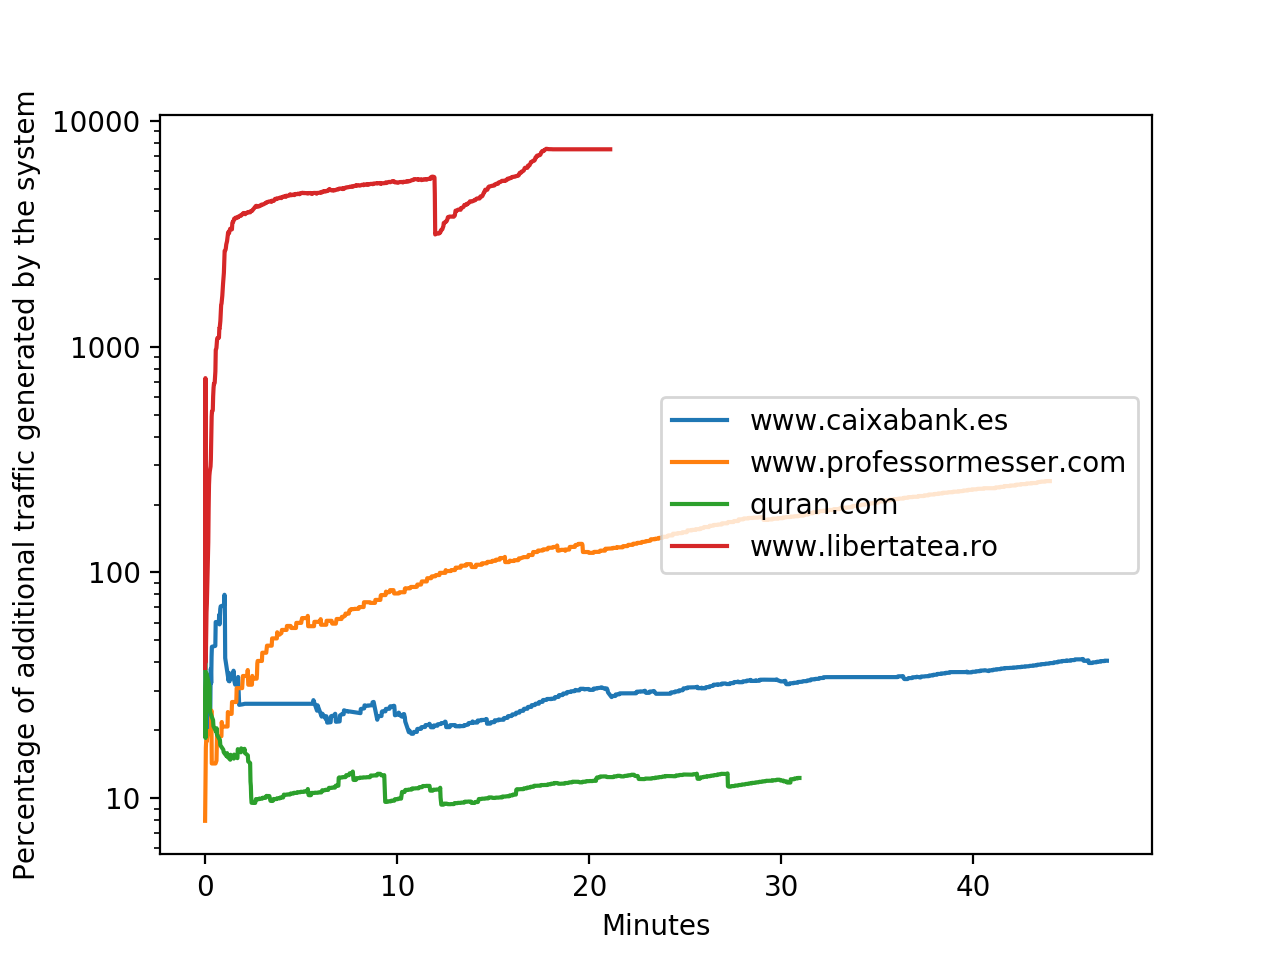
\includegraphics[width=\textwidth]{imgs/netword_usage_plot.png}
	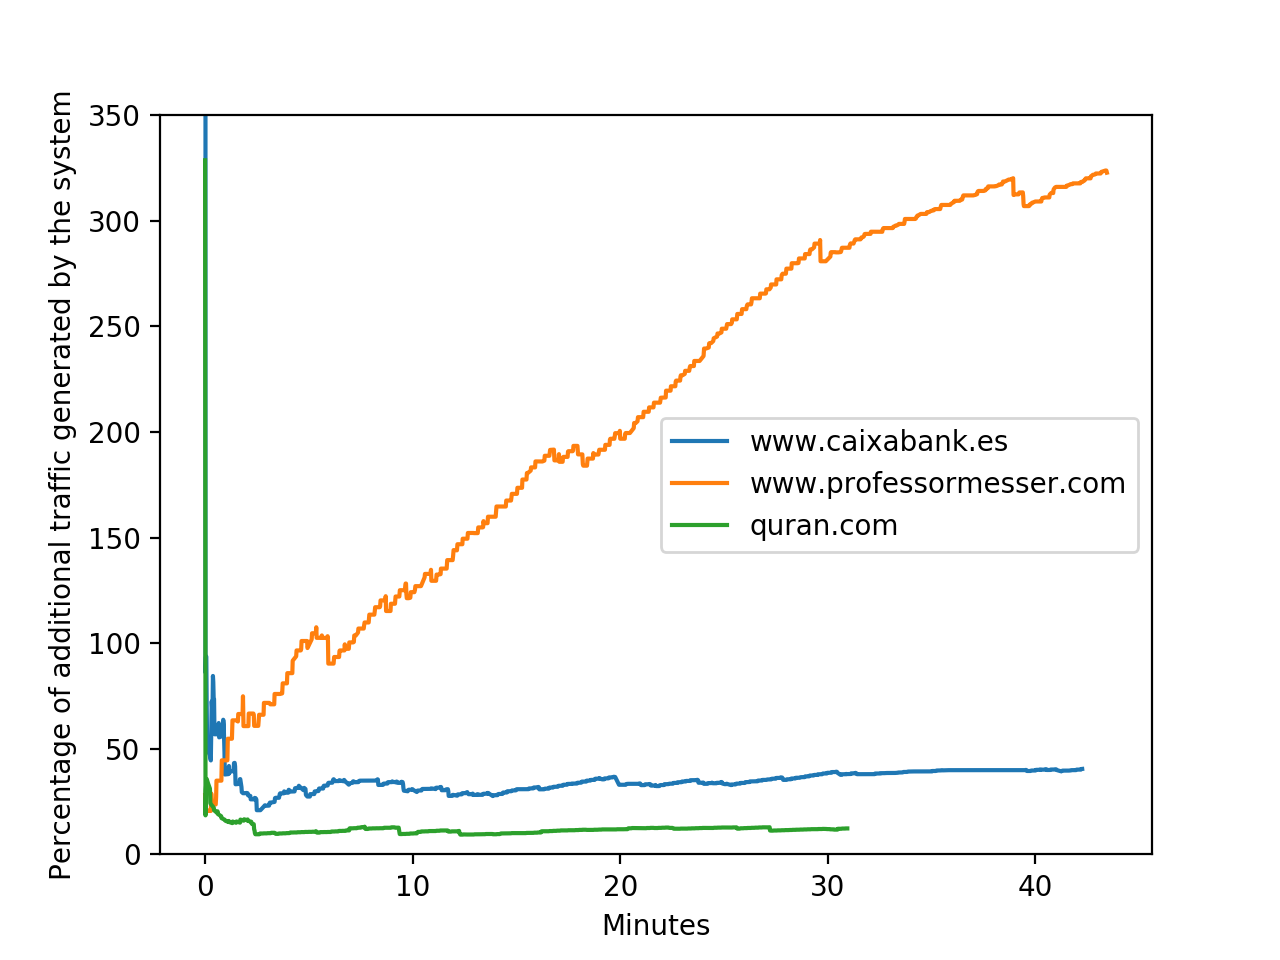
\includegraphics[width=\textwidth]{imgs/netword_usage_long_plot.png}
	\caption{Percentage of bandwidth dedicated to additional traffic generated by the Policy Maker using default settings}
	\label{fig:standarUsage}
\end{figure}

Table \ref{tab:optimistic} shows many reports and policy related statistics.
Percentage traffic added to header signifies the unavoidable increase in data transferred which is on the critical path to the user.
As the policies, sizes of which are also displayed in this table, need to be sent in the header of the response.
This means that they will be received by the user before any other content, increasing the time before the site is responsive.

The Policy Maker was also tested with the host added to the csp from the start.
This scenario ignores scripts loaded from the host, but still checks all inline and external scripts.
When adding this source, the site is no longer protected from insider threats or reflected attack where a malicious script is saved to the host.
The server still protects from many common DOM injections and depency hosts turning malicious.
The restults of this test are shown in table \ref{tab:percentageBypass}.
As shown the results are much better where additional traffic to Caixabank has reduced from 12\% to 8\%, making the Policy Maker even more viable.
Quran.com uses no sources outside of itself and in this example the 4\% is the minimal load increase that is required for the system to function.
\begin{table}
\begin{center}
\begin{tabular}{| c c c c |}
	\hline
	Host & Total Host Traffic & Additial Traffic & Percentage Added \\ \hline
	www.caixabank.es        & 378.6 MB & 31.9 MB &   8\% \\ \hline
	quran.com               &  18.8 MB &  0.7 MB &   4\% \\ \hline
	www.professormesser.com &   3.1 MB &  8.0 MB & 261\% \\ \hline
	www.libertatea.ro       &   8.0 MB & 30.4 MB & 382\% \\ \hline
\end{tabular}
\end{center}
\label{tab:percentageBypass}
	\caption{Final network usage statistics when scripts from the host are allowed}
\end{table}



The costs detailed in both tables should be carefully examined by the potential users of the Policy Maker.
The automated tool provied a significant boost to security by reducing the time to detect any attacks.
It also has not insignificant monetary and experience costs associated to running the server.

% \section{Discussion}
% Maybe TODO
% What is a good time to forget the link

\section{Things to improve}

The approach shown in this paper proves to be a new and promising way to improve the security of particular websites.
Main applicability issues stem from the quickly expanding and untamed environment of front end development.
Websites may quickly grow to sizes which prove to be unmenagable by the Policy Maker.

\subsection{Content-Security-Policy Specificaiton Changes}

During the development of the Policy Maker, it had to comply with the Content-Security-Policy specification.
This results in issues and small insecurities, which could be solved if the specification was more robust.

\subsubsection{Variable reports}

Things that could dramatically improve the performance of the Policy Maker would require changing the CSP standard.
Allowing for more control over the report template could reduce the data transferred back to the CSP reporting endpoint by about 90\%.
This comes from each report containing the current policy used when loading the page, which is responsible for most of the traffic.
For each host this percentage is displayed in table \ref{tab:reduction}.
With significant reduction in report sizes, the project would operate much lower overheads.
This idea could be implemented by creating a new directive \texttt{report-fields} where each source of type \texttt{'no-original-policy'} or \texttt{'no-violated-directive'} would prevent the specific field from being included in the report.
This solution will work with CSP idea of backwards compatibility as older browser will ignore this directive and send full reports.

\begin{table}[h]
\begin{center}
\begin{tabular}{| c c |}
	\hline
	Host & Bytes used by Original Policy in Reports \\ \hline
	www.caixabank.es        & 95 \% \\ \hline 
	quran.com               & 85 \% \\ \hline 
	www.professormesser.com & 90 \% \\ \hline 
	www.libertatea.ro       & 95 \% \\ \hline 
\end{tabular}
\end{center}
	\caption{How much of each report is the current policy}
\label{tab:reduction}
\end{table}



% Bytes used by Policy in Reports & 
% 95 \% &
% 85 \% &
% 90 \% &
% 95 \% &
%
%          host           | maxPolicy | justpolicy | percentage 
%-------------------------+-------+------------+------------
% quran.com               |      3462 |    1262625 |         85
% www.professormesser.com |      5740 |    7100481 |         90
% www.caixabank.es        |     15184 |   28999240 |         95
% www.libertatea.ro       |     41440 |   25550687 |         95





\subsubsection{Script hash in reports}

Another useful addition to the CSP reports specification would be the possibility to ask the browser to pass the hash of the loaded scripts.
It would allow the oracle to check whether the retreived script is identical to the one that the user has loaded.
Currently, even if the oracle succesfully retreives a scripts there is no such guarantee and the script may have changed in between.
The loss of privacy incured by adding hash is either very negligible or non existent as reports are already passing full url of blocked resources and sites on which said violation happened.
This feature could be implemented in a similar way to \texttt{report-sample} source, where \texttt{report-hash} would send the hash of the script as received by the browser.

\subsubsection{Looser integration checks}

The project initially intended to use hashes for each type of script. 
This would potentially allow for scripts to be checked before timeout by receiving a significant amount of reports when it no longer has the previously calculated hash.
Unfortunately, the CSP standard required integration attribute for \texttt{<script>} elements which are loaded from a file \cite{externalHash}.
The integration attribute needs to contain the expected hash, which also needs to match a hash in the CSP for the script to be loaded.
Adding such attribute nullifies the idea of a automatic tool, that could work independeently from the rest of the codebase.
Due to this reason the server uses a mixture of url and hash based allowlists, lowering the security slightly.

To make the described approach work, the specification would need to make a way to ingore the integration attribute and check the hashes after the script is loaded.
This would not change the behaviour of the browser when using the report only policy as the non enforcing nature allows all scripts to be laoded.
When used with the enforcing policy it would allow for data to be sent out of and received by the browser, before potentially blocking the script.
As CSP is not particularly good at preventing exfiltration attacks \cite{CSPexfil}, such addition would allow to balance security and usability of CSPs.

Unfortunately, this specification change would break the backwards compatibility the most out of all proposed changes within this paper.
When used in enforcing mode, older browsers which are not updated to use this feature, would block otherwise allowed cources from executing.
In report only mode, it would result in many bogus reports, which would either be ignored or significantly strain the system.
Although this change would severely increase the security of the Policy Maker, it is unlikely to be added, due to issues described above.

\subsection{Other improvements}

\subsubsection{Real life deployment}

Within the impact estimation, the server is tested on existing codebases of real hosts.
This is the closest this set of tests can go, without being actually integrated into the server itself.
The next logical step for the Policy Maker is to be tested alongside a willing host.
This would allow to calculate the real impact of the server by receiving reports from the website's users.
It would also show any issues with the Policy Maker logic, when reports received are old, invalid or from a varying set of browsers.

\subsubsection{Evaluator Improvements}

The evaluator in this project is a rather simple machine learning model which functions great for testing and development purposes.
It could be expanded by using more data when deciding the maliciousness of the script.
It could include hostnames and IP adresses and compare those agains a set of known compromised endpoints.
It could also benefit from more training data or from more elaborate lignuistic models.
The possibilities to improve the evaluator are many and they should be seriously considered when trying to run the Policy Maker on a real host.

\subsubsection{Securing other Frames and Styles}

This work focues on protecting against JavaScript based attacks, while giving some insight into iframes that are embedded within the site.
Protecting against attacks using either of those elements is much harder because of prectical reasons.
As sites are moving away from using inline attribute scripts, styles can still be commonly found in attributes of many html elements.
Attacks using styles are also much harder to detect as they often retreive single characters at a time.
This would result in big policies with potentially little benefit to them.

IFrames on the other hand require more context to be considered malicious.
A payment IFrame is to be expected on a shopping site, but the same iframe may be considered malicious when injected into the landing page of a IT solutions provider, which does not work with individual clients.
For this reason the server implemented in this work displays the iframes encountered as warnings, as each frame should be reviewed manually.

